\documentclass[a4paper,UTF8]{article}
\usepackage{ctex}
\usepackage[margin=1.25in]{geometry}
\usepackage{color}
\usepackage{graphicx}
\usepackage{amssymb}
\usepackage{amsmath}
\usepackage{amsthm}
%\usepackage[thmmarks, amsmath, thref]{ntheorem}
\theoremstyle{definition}
\newtheorem*{solution}{Solution}
\newtheorem*{prove}{Proof}
\usepackage{multirow}
\usepackage{url}
\usepackage{enumerate}
\usepackage{algorithm}
\usepackage{algorithmic}
\usepackage{caption}
\usepackage{subcaption}
\usepackage{booktabs}
\usepackage{listings}
\bibliographystyle{plain}
\renewcommand\refname{参考文献}


%--

%--
\begin{document}
\title{MapReduce课程设计}
\author{周华平,蒋雅楠,高翼枭}
\maketitle

\section*{小组信息}

\begin{table}[htbp]
  \centering
  \begin{tabular}{l|l|l|l|l}
	\hline
	学号 & 姓名 & 邮箱 & 导师 & 研究领域 \\
	\hline
	MG1733098 & 周华平 & \url{zhp@smail.nju.edu.cn} & 田臣 & 数据中心网络 \\
	MF1733026 & 蒋雅楠 & \url{mf1733026@smail.nju.edu.cn} & 田臣 & 数据中心网络 \\
	DZ1733004 & 高翼枭 & \url{dz1733004@smail.nju.edu.cn} & 田臣 & 数据中心网络 \\
	\hline
  \end{tabular}
\end{table}

\section*{课题分工}

本课题的选题和讨论由三人共同完成;
项目的代码部分包含多个MapReduce Job。
具体分工如下:

\begin{table}[htbp]
  \centering
  \begin{tabular}{l|l}
	\hline
	姓名 & 主要工作 \\
	\hline
	周华平 & 整体架构设计;各Job中流程设计与实现 \\
	蒋雅楠 & 文件输入输出;Distributed Cache使用 \\
	高翼枭 & 数据连接;HDFS读取、写入、删除文件 \\
	\hline
  \end{tabular}
\end{table}

\section*{课程设计题目}

我们研究的题目为“基于近邻成分分析的距离度量学习算法的并行化”。
该题目来源于实现高级机器学习作业的过程中遇到的实际问题:
在样本数据量较大或者维度较高的情况下,
由于计算和存储开销较大,在单机上无法执行全梯度下降,
因此该算法需要使用随机梯度下降代替常规的梯度下降来完成计算,
这可能会导致算法无法正确收敛。

因此,在本课题中我们计划使用MapReduce对NCA算法进行并行化,
使得该算法能够完整地运行在在较高维度和较大规模的数据集上,
并且能够缩短训练时间。

\section*{摘要}

本次课题,我们基于对度量学习过程中大量计算的并行化想法,来设计MapRedue任务。
实现算法采用近邻成分分析,并使用梯度下降法求解目标函数。
由于算法的数据量较大,而且需要计算任意样本对当前分类样本的影响,
求取样本被正确分类的最大概率,对计算与存储的要求都很高。
于是我们将这样一个算法拆解成若干个MapReduce Job,建立一个具有依赖关系的任务链。
首先计算各个样本间的距离$x_{ij}$并写出至文件,便于下次使用;
将需要更新的矩阵A放入Distributed cache中,便于各个节点读取操作;
根据已得到的$x_{ij}$与矩阵A求解样本分类影响$p_{ij}$和$p_{i}$并输出;
再利用中间结果进行数据连接计算$p_{ij} x_{ij} x_{ij}^\top$。
然后可以通过简单操作得到当前梯度,更新矩阵A,并进入下一轮迭代,
直至A的变化小于某一阈值,或达到迭代次数终止。

\section*{研究问题背景}

在机器学习领域中,如何选择合适的距离度量准则一直都是一个重要而困难的问题。
因为度量函数的选择非常依赖于学习任务本身,并且度量函数的好坏会直接影响到学习算法的性能。
为了解决这一问题,我们可以尝试通过学习得到合适的度量函数。
距离度量学习(Distance Metric Learning, DML)的目标是学习得到合适的度量函数,
使得在该度量下更容易找出样本之间潜在的联系,进而提高那些基于相似度的学习器的性能。

在本课题中,我们采用近邻成分分析(Neighbourhood Component Analusis, NCA)来实现距离度量学习,

\subsection*{度量函数学习目标}

根据马氏距离的定义
\[
	dist_{mah}^2(x, y) = (x - y)^\top Q(x - y) = (Ax - Ay)^\top (Ax - Ay)
\]
其中$Q$称为“度量矩阵”,而DML则是对$Q$的学习。
为了保持距离非负且对称,$Q$必须是(半)正定对称矩阵,即必有正交基$A$使得$Q$能写为$Q = AA^\top$。

为了提高近邻分类器的性能,我们将$Q$直接嵌入到近邻分类器的评价指标中去,
通过优化该性能目标相应地求得$Q$。
在本实验中我们采用近邻成分分析进行学习。

近邻分类器在进行判别时通常使用多数投票法,领域中的每个样本投1票,
领域外的样本投0票。NCA将其替换为概率投票法,对于任意样本$x_{j}$,它对$x_{i}$分类结果影响的概率为
\[
	p_{ij} = \frac{\exp(-\lVert Ax_{i} - Ax_{j} \rVert^2)}
	{\sum_{k \neq i} \exp(-\lVert Ax_{i} - Ax_{k} \rVert^2)}, \qquad
	p_{ii} = 0
\]
若以留一法正确率的最大化为目标,则可计算$x_{i}$的留一法正确率,
即它被自身之外的所有样本正确分类的概率为
\[
	p_{i} = \sum_{j \in C_{i}} p_{ij}
\]
其中$C_{i} = \lbrace j \vert c_{i} = c_{j} \rbrace$,
即与$x_{i}$属于相同类别的样本的下标集合。
于是,整个样本集上被正确分类的点的个数的期望为
\[
	f(A) = \sum_{i} \sum_{j \in C_{i}} p_{ij} = \sum_{i} p_{i}
\]

NCA的优化目标是使得$f(A)$最大化,即
\[
	\max_{A} \sum_{i} \sum_{j \in C_{i}}
	\frac{\exp(-\lVert Ax_{i} - Ax_{j} \rVert^2)}
	{\sum_{k \neq i} \exp(-\lVert Ax_{i} - Ax_{k} \rVert^2)}
\]

\subsection*{优化算法}

梯度下降法可以用来求解目标函数:
通过求$f$对$A$的偏导,可以得到梯度公式(令$x_{ij} = x_{i} - x_{j}$)
\[
	\frac{\partial f}{\partial A} =
	-2A \sum_{i} \sum_{j \in C_{i}}
	p_{ij}( x_{ij} x_{ij}^\top - \sum_{k} p_{ik} x_{ik} x_{ik}^\top)
\]
根据该公式,使用梯度下降法即可求解NCA的目标函数。
得到最大化近邻分类器留一法正确率的距离度量矩阵$Q$。

\section*{主要技术难点和拟解决的问题}

在高级机器学习课程中,我们使用了Python实现了该算法。
在该实现中,为了尽可能利用numpy高效的矩阵操作,
我们需要将中间结果的计算尽可能转化为矩阵的运算,从而提高并行度。
然而当样本的维度较高或者样本数据量较大时,
无论是存储中间结果矩阵还是计算梯度的开销都会大到单机无法承受的程度。

因此,在实际实验中我们会用随机梯度下降来代替全梯度下降,
即以计算梯度中的某些项来代替梯度全体,以此降低计算和存储开销。
然而随机梯度下降并不是保证迭代将沿着目标函数的最快下降方向前进,
甚至不保证其沿着下降方向前进。
这有可能导致算法收敛过慢、无法正确地收敛、以及在接近最优解附近时精度较差等问题。

在本课题中我们计划使用MapReduce来完成NCA算法中梯度下降的并行化,
使其在能够处理维度较高、数据量较大的样本训练的同时缩短训练时间。

该算法需要使用多个MapReduce作业,通过迭代的方式完成计算。
对$\frac{\partial f}{\partial A}$的计算分为了几个阶段,
我们需要将其中的计算抽象为若干个MapReduce过程,
合理地设计每个阶段的输入和输出,并将不同阶段组织成具有依赖关系的任务链;
在中间结果的计算中还需要涉及多数据源的连接。
简单来说,我们首先得到样本间的距离文件$x_{ij}$和初始矩阵A,
然后可以利用MapReduce并行地计算$\exp(-\lVert Ax_{i} - Ax_{j} \rVert^2)$,
此处并行可以大量减少计算时间;
接着将该结果作为输入,可以并行地计算$p_{ij}$和$p_{i}$;
利用上述中间结果,我们可以通过DataJoin来计算$p_{ij} x_{ij} x_{ij}^\top$;
最后计算出当前的$\frac{\partial f}{\partial A}$并更新矩阵$A$,完成一次迭代。

\section*{基本解决方法和设计思路}

\subsection*{NCA模型训练}

对于NCA,我们拟采用组合式MapReduce计算作业来实现。
由于梯度下降法需要用迭代方法求得逼近结果,
因此在NCA的主控程序中,需要使用一个循环来控制MapReduce作业的执行,
直到第$n$次迭代后结果与第$n-1$次的结果小于某个指定的阈值时结束,
或者通过经验值可确定在运行一定的次数后能得到接近的最终结果,
也可以控制循环固定的次数。

对于梯度下降中需要求解的变量,
我们采用顺序组合式MapReduce作业来依次计算:
首先我们可以通过DataJoin对集合$X$做笛卡尔积,
进而可以计算出$x_{ij}$;
在此基础上以$x_{ij}$与矩阵A作为输入,
我们可以进一步执行MapReduce任务计算出中间结果r1:
$\exp(-\lVert Ax_{i} - Ax_{j} \rVert^2)$,
其中矩阵$A$作为Distributed Cache在Mapper的setup()阶段读入;
基于以上结果,我们可以通过下一次MapReduce任务对所有$i$计算出中间结果r2:
$\sum_{k \neq i} \exp(-\lVert Ax_{i} - Ax_{k} \rVert^2)$,
再通过DataJoin连接上述两个中间结果r1与r2,我们可以计算出$p_{ij}$。

$p_i$的计算需要考虑$x_j$与$x_i$的label是否相同。
因此我们可以通过接下来的MapReduce任务,
在setup()中读入distributed cache中的lable文件,
生成一个i与lable的映射表,
并通过Mapper过滤掉$x_j$与$x_i$label不同的元素,
在Reducer端只需做简单的求和即可。

基于以上数据,我们可以对梯度$\frac{\partial f}{\partial A}$进行求解。
我们首先使用DataJoin计算出中间结果$p_{ij} x_{ij} x_{ij}^\top$,
然后使用不同的Mapper过滤元素,分别计算
$\sum_{k} p_{ik} x_{ik} x_{ik}^\top$以及$\sum_{j \in C_i} p_{ij} x_{ij} x_{ij}^\top$,
需要注意的是由于这两者的计算没有依赖关系,所以可以通过配置Job使它们并行执行。
在计算出以上两个求和的结果后,
梯度$\frac{\partial f}{\partial A}$可以通过简单的运算操作得出,这里不做赘述。
在每次迭代的最后,我们利用当前位置的梯度对矩阵$A$进行更新,并启动下一次迭代。

\section*{详细设计说明}

\subsection*{自定义数据类型}

\subsubsection*{MatrixWritable}

由于NCA中涉及了大量的矩阵运算,为了更加方便和效率地存储和表示矩阵,
我们实现了MatrixWritable类。
该类实现了Writable接口,能够对矩阵进行序列化和反序列化。
MatrixWritable底层使用math3.linear.RealMatrix来表示矩阵,
该类来自于commons-math3包,它提供了一系列矩阵相关的操作。
NCA中大部分的中间结果都采用MatrixWritable来表示和存储。

\subsubsection*{TaggedEntry}

在使用DataJoin时,DataJoinMapperBase默认会忽略map函数的key参数,
而将GroupKey作为输出的Key。
这样做的问题在于当处理SequenceFile或者其他Key-Value类型的输入数据时,
Key参数在map阶段就会被丢弃。

针对这种情况,我们实现了TaggedEntry基类,
它继承自TaggedMapOutput基类,
将Key也作为序列化数据的一部分,
这样在Reducer端除了GroupKey以外,记录的Key依旧能够得到保留。
TaggedMatrix继承了该类,它的Value类型为MatrixWritable。

\subsection*{中间数据格式}

由于NCA采用了组合式MapReduce计算作业来实现,程序需要多趟迭代,
每一趟又由多个Job串联而成,因此对于中间结果我们需要使用更高效的方式来存储。
为此我们使用SequenceFile作为中间数据的文件格式,
其中Key类型为Text,Value类型为MatrixWritable。
Key总共有两种形式:对于类似$p_{ij}$的中间数据,Key为``i,j''这样的值对,
中间用逗号分隔;对于类似$p_{i}$的中间数据,Key为``i''。

\subsection*{功能模块}

在NCA中的涉及的运算主要可以分为3类。
首先是输入和输出一一对应的情况。例如根据$x_{ij}$计算$x_{ij} x_{ij}^\top$。
对此我们只需要对每种运算分别实现一个Mapper即可。
例如XXtMapper和ExpSquaredNormMapper
分别用于计算$x_{ij} x_{ij}^\top$和$\exp(-\lVert Ax_{i} - Ax_{j} \rVert^2)$,

其次是输出对输入聚合的情况。
例如根据$p_{ij}$计算$p_{i} = \sum_{j \in C_{i}} p_{ij}$。
这种是典型的MapReduce的应用:我们使用Mapper对输入进行过滤(Filter),
然后在Reducer端对结果进行聚合。

由于在程序中多次使用到了类似的编程范式,因此我们对于这些算子进行了进一步的抽象。
具体说来,GroupMapper将KEYIN``i,j''中的i作为map()函数的KEYOUT,
而SameLabelMapper则会忽略掉那些$y_i \neq y_j$的元组,
即Mapper输出的结果必定具有相同的Label。
对于这类运算我们仅实现了SumMatReducer这一种Reducer。
通过Mapper和Reducer的不同组合,我们可以实现不同的运算。
例如使用SameLabelMapper和SumMatReducer
即可计算$\sum_{j \in C_{i}} p_{ij}$;
而使用GroupMapper和SumMatReducer即可计算$\sum_{k} p_{ik} x_{ik} x_{ik}^\top$。

最后一类是输出需要连接多个输入源的情况。
例如根据$p_{ij}$和$x_{ij} x_{ij}^\top$来计算$p_{ik} x_{ik} x_{ik}^\top$。
为此我们使用DataJoin来进行多数据源的连接。
由于在NCA中我们主要使用二元连接操作,因此我们对这种情况进行了特殊的处理,
将输入源分为了Left和Right,代表运算符两边的操作数。
我们实现了EntryJoinMapperBase基类,
它继承自DataJoinMapperBase。
我们通过configure()读取在Configuration中设置的Left和Right对应的文件名,
在此基础上我们重载了generateInputTag(),
根据inputFile的路径判断该分片是属于Left还是Right,并设置相应的Tag。
除此之外,我们还需要修改map(),使得Key能够通过TaggedEntry来保留。
至此我们就能够将输入源打上Tag并发送到Reducer端。
并且由于Reducer端接收到的元组会根据它们的Tag进行排序,
我们可以很容易地通过巧妙设置Tag的字面值,达到在Array中Left必定在Right前面的效果,
所以在Reducer端不需要判断Tag的字面值而可以直接使用变量值。

在EntryJoinMapperBase的基础上,
我们分别实现了DefaultMapper和GroupMapper。
其中GroupMapper和用于聚合的GroupMapper具有相似的作用,
而DefaultMapper将元组的Key直接作为GroupKey。

通过继承EntryJoinReducerBase,我们实现了连接端不同的矩阵运算操作:
例如NumMulMatReducer和MatSubReducer
分别实现了数乘矩阵和矩阵减法操作。

通过组合使用EntryJoinMapperBase和EntryJoinReducerBase,
我们可以实现各种矩阵的二元运算,这直接体现在了代码中,这里就不过多赘述。

\subsection*{程序框架说明}

上一节中所介绍的第一和第二类运算相关的实现位于NCA类中;
而第三类运算的实现位于MatJoin类中。
NCADriver类负责对输入参数进行处理并调度MapReduce Job的执行。
NCADriver在开始执行时会调用一次init(),
用于对输入数据转化为SequenceFile格式,然后计算$x_{ij}$和$x_{ij} x_{ij}^\top$,
将以上输出结果保存到HDFS中以供后续训练使用。这样能省去许多重复计算。

接下来NCADriver每调用一次train()都会调度一系列MapReduce Job
来计算梯度,最后将结果累加到$A$上并保存到HDFS上,从而完成一趟训练。

\section*{输入输出文件格式}

\subsection*{输入文件格式}

输入文件均为文本文件,其中一个是$x_{ij}$,即$x_i - x_j$。
其每行的格式为i,j$\backslash$t$x_i[0]-x_j[0] \dots x_i[n]-x_j[n]$,
向量中的每个值用空格分隔;

另一个输入文件是$y_i$,即每个元组的标记信息。
其每行的格式为i$\backslash$t$label_i$。

\subsection*{输出文件格式}

输出的数据是训练得到的距离度量矩阵$A$,它是一个二进制文件,
通过使用Utils.serializeMatrix()和Utils.deserializeMatrix()
可以对其进行序列化和反序列化操作。

\section*{程序运行实验结果和说明分析}

为了测试NCA的性能,我们使用一个包含1000条数据的数据集,其中每条数据的维度为16。
通过提交到集群执行,我们观察到每一趟训练产生的中间结果可以达到将近10G,
这还是在输入数据量不是很大的情况下得到的结果,
我们能够很明显感受到维度爆炸带来的影响:这样的数据量很难在单机上有效处理。

\subsection*{运行方式说明}

我们通过以下命令执行NCADriver。其中raw\_x\_ij.txt代表文本文件$x_{ij}$;
label.txt代表文本文件$y_i$;dim代表数据维度;train代表工作目录;
matA代表矩阵$A$所在的路径;lr代表学习率;epoch代表迭代轮数。

\begin{lstlisting}
hadoop jar nca.jar nca.NCADriver
	raw_x_ij.txt label.txt dim train matA lr epoch
\end{lstlisting}

\begin{figure}[H]
	\centering
	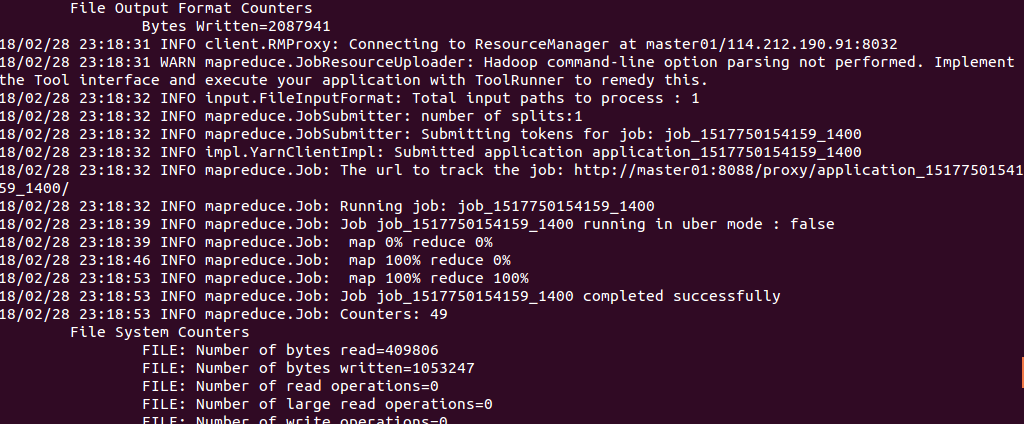
\includegraphics[width=\textwidth]{pic/run.png}
	\caption{部分执行过程}
\end{figure}
\begin{figure}[H]
	\centering
	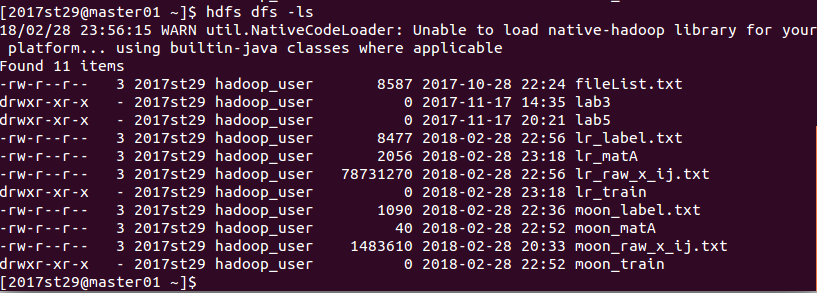
\includegraphics[width=\textwidth]{pic/hdfs.png}
	\caption{HDFS文件列表}
\end{figure}

\subsection*{程序执行报告}

以下为某一趟训练产生的Job的执行报告。

\begin{figure}[H]
	\centering
	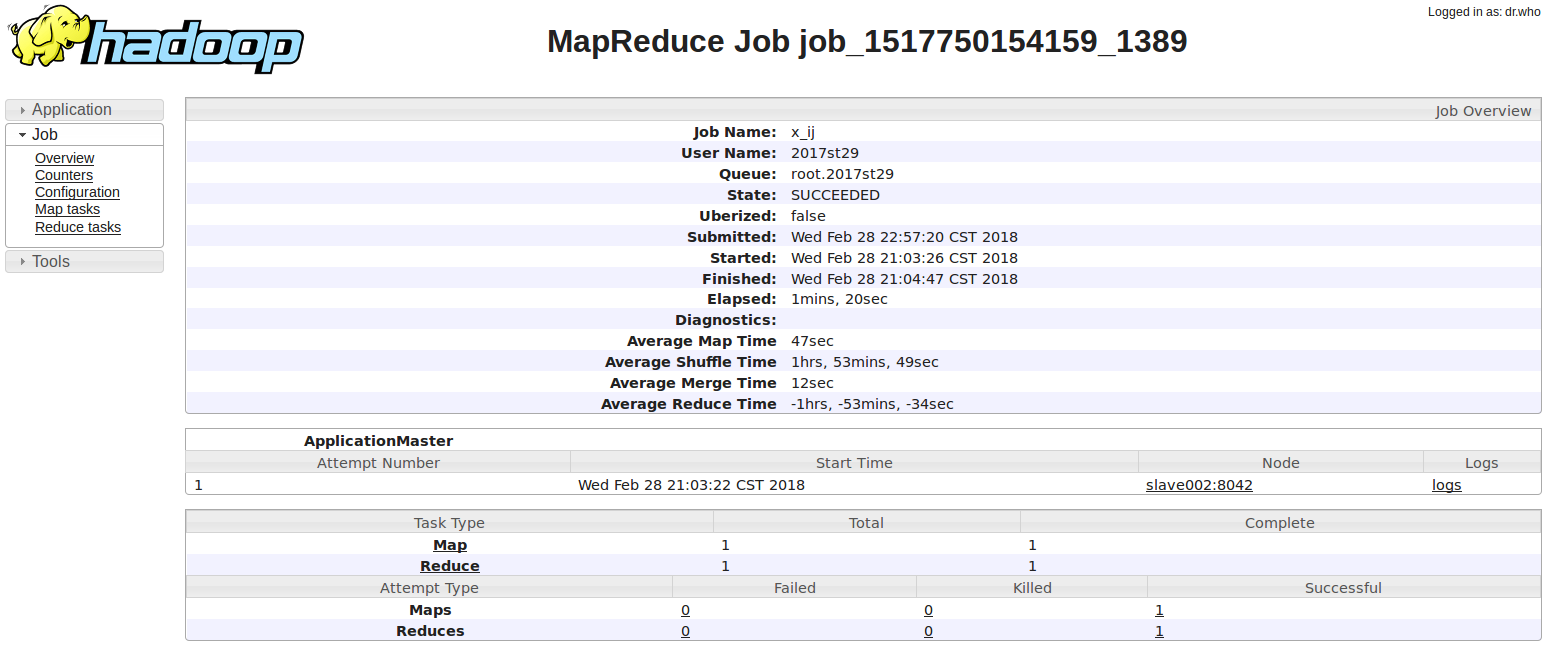
\includegraphics[width=\textwidth]{pic/389_x_ij_job.png}
	\caption{x\_ij Job}
\end{figure}
\begin{figure}[H]
	\centering
	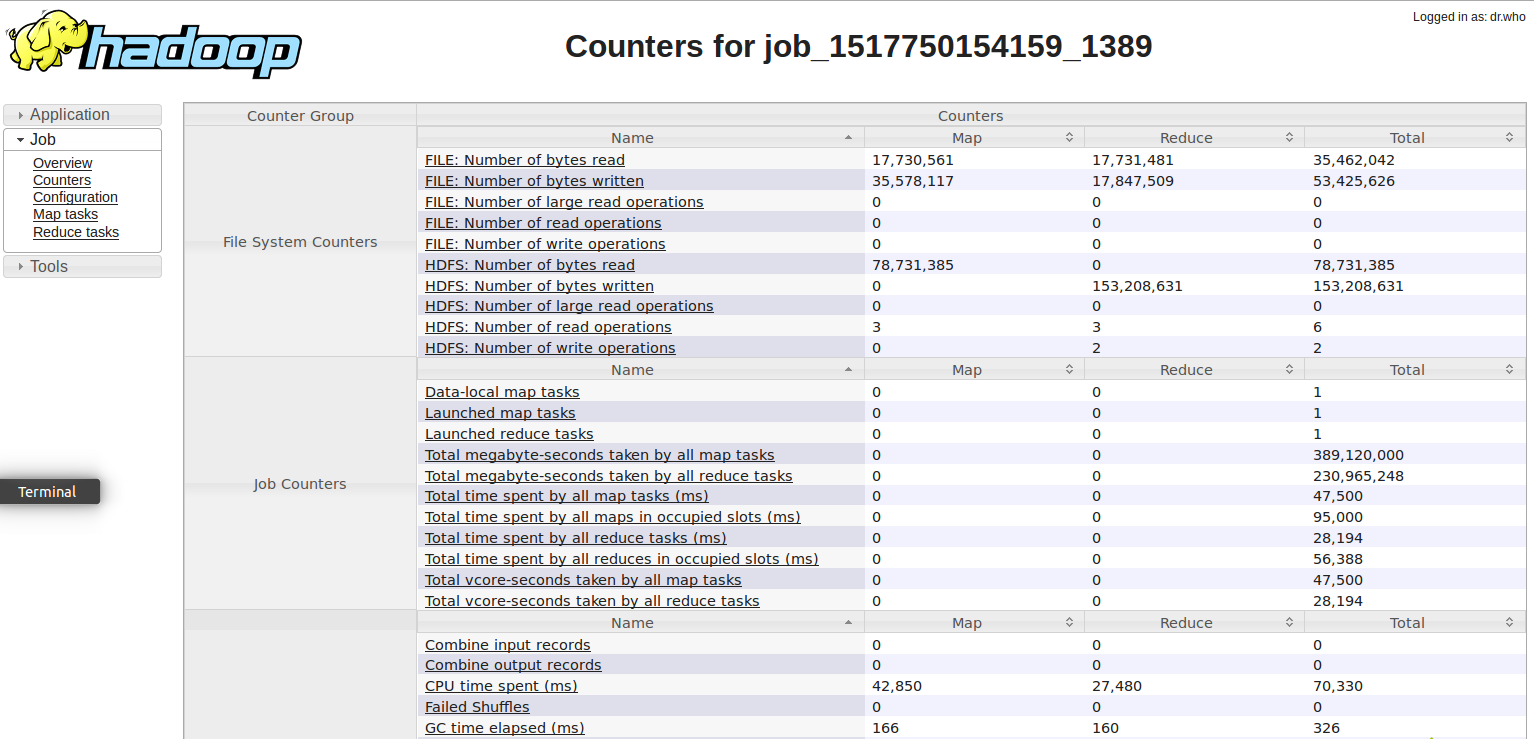
\includegraphics[width=\textwidth]{pic/389_x_ij_counters.png}
	\caption{x\_ij Counters}
\end{figure}

\begin{figure}[H]
	\centering
	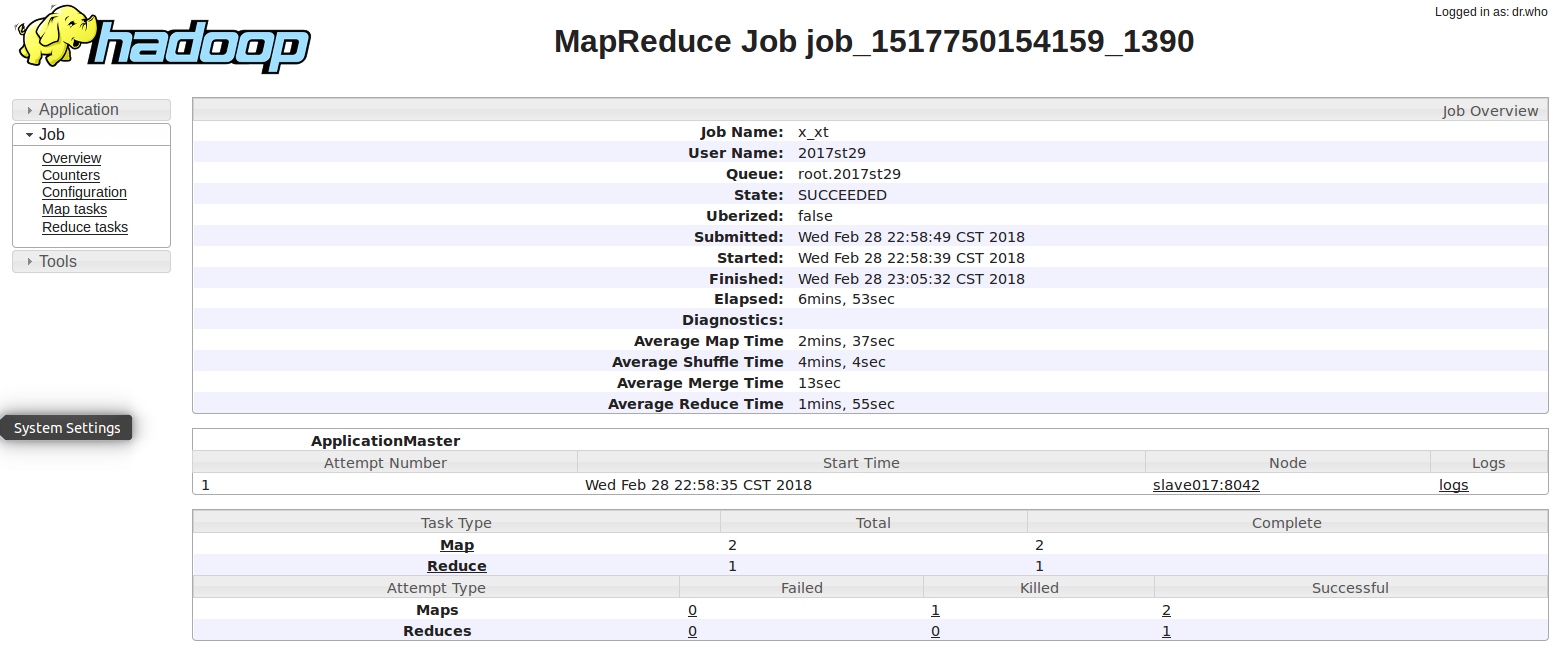
\includegraphics[width=\textwidth]{pic/390_x_xt_job.png}
	\caption{x\_xt Job}
\end{figure}
\begin{figure}[H]
	\centering
	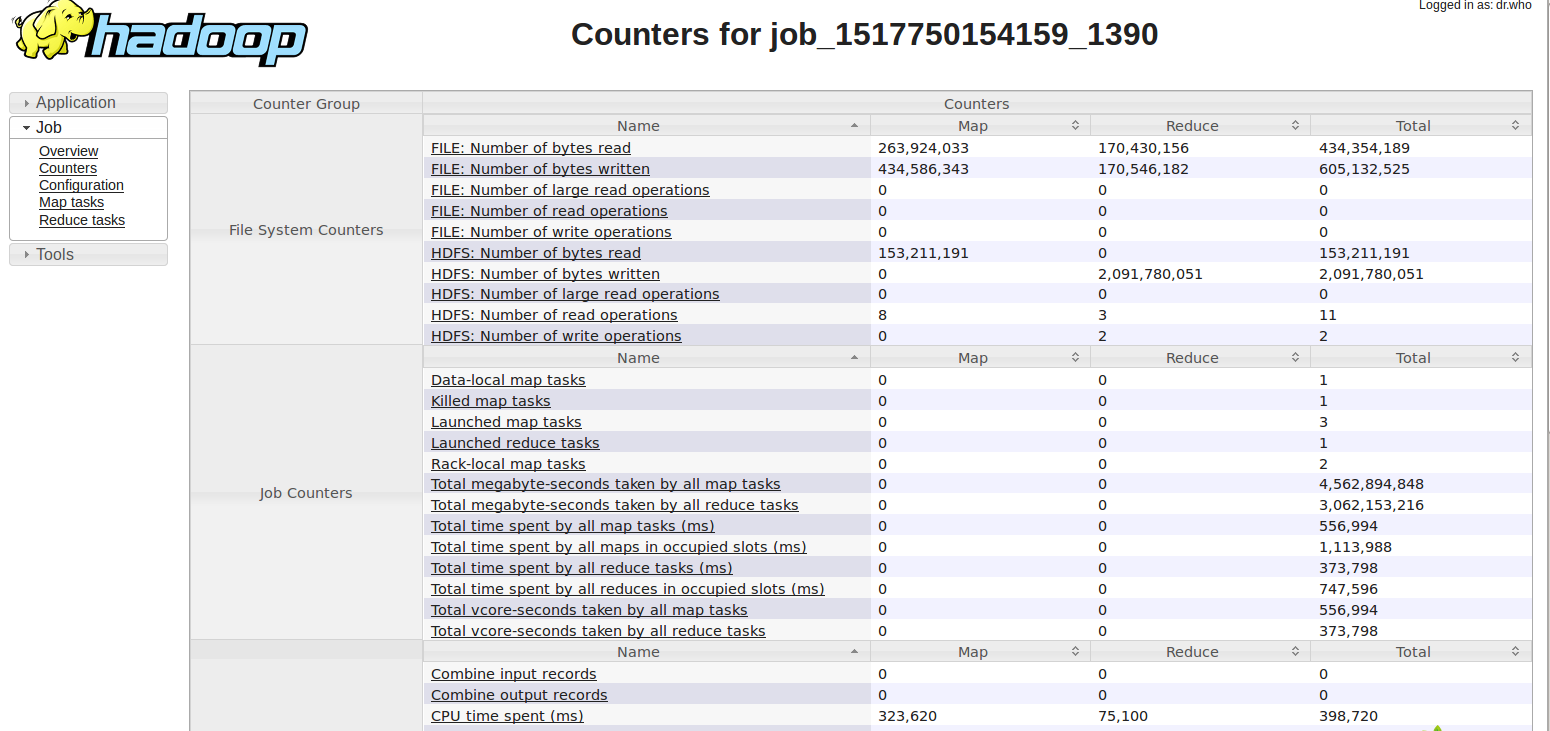
\includegraphics[width=\textwidth]{pic/390_x_xt_counters.png}
	\caption{x\_xt Counters}
\end{figure}

\begin{figure}[H]
	\centering
	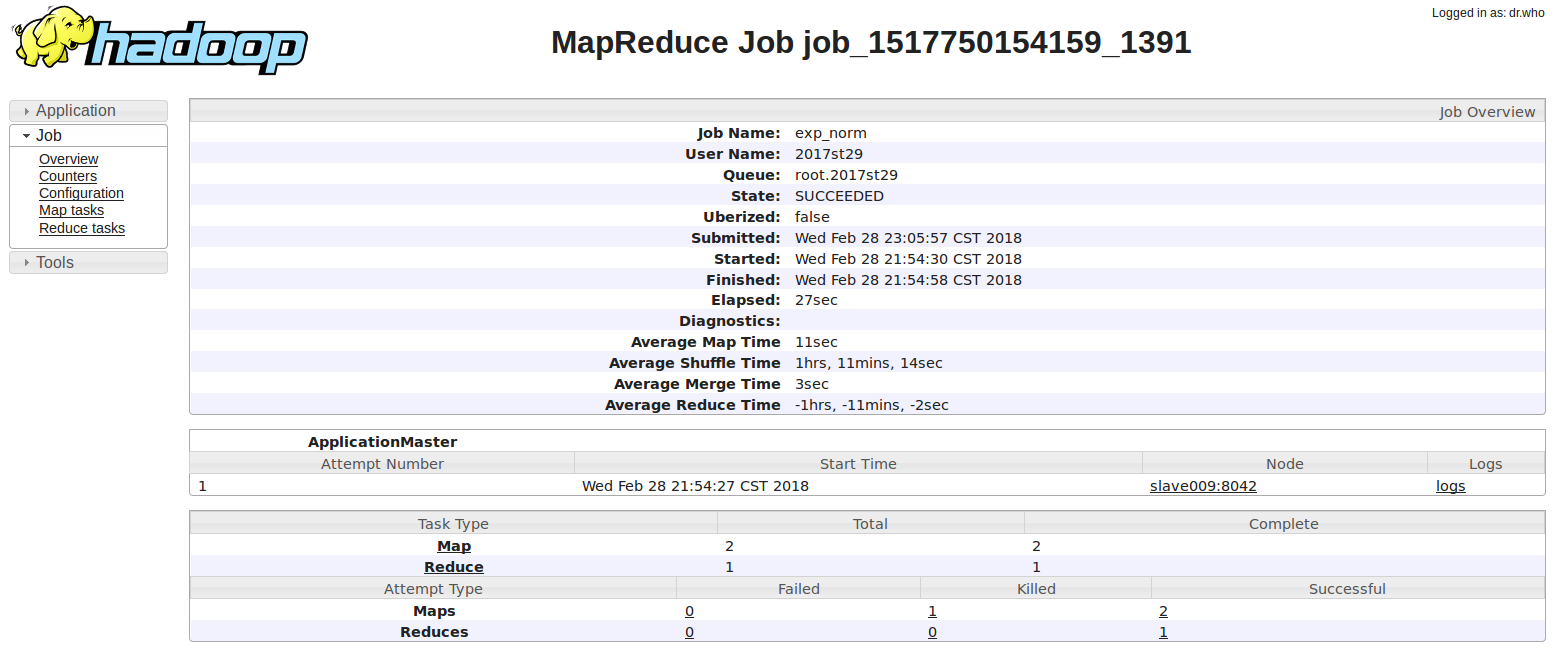
\includegraphics[width=\textwidth]{pic/391_exp_norm_job.png}
	\caption{exp\_norm Job}
\end{figure}
\begin{figure}[H]
	\centering
	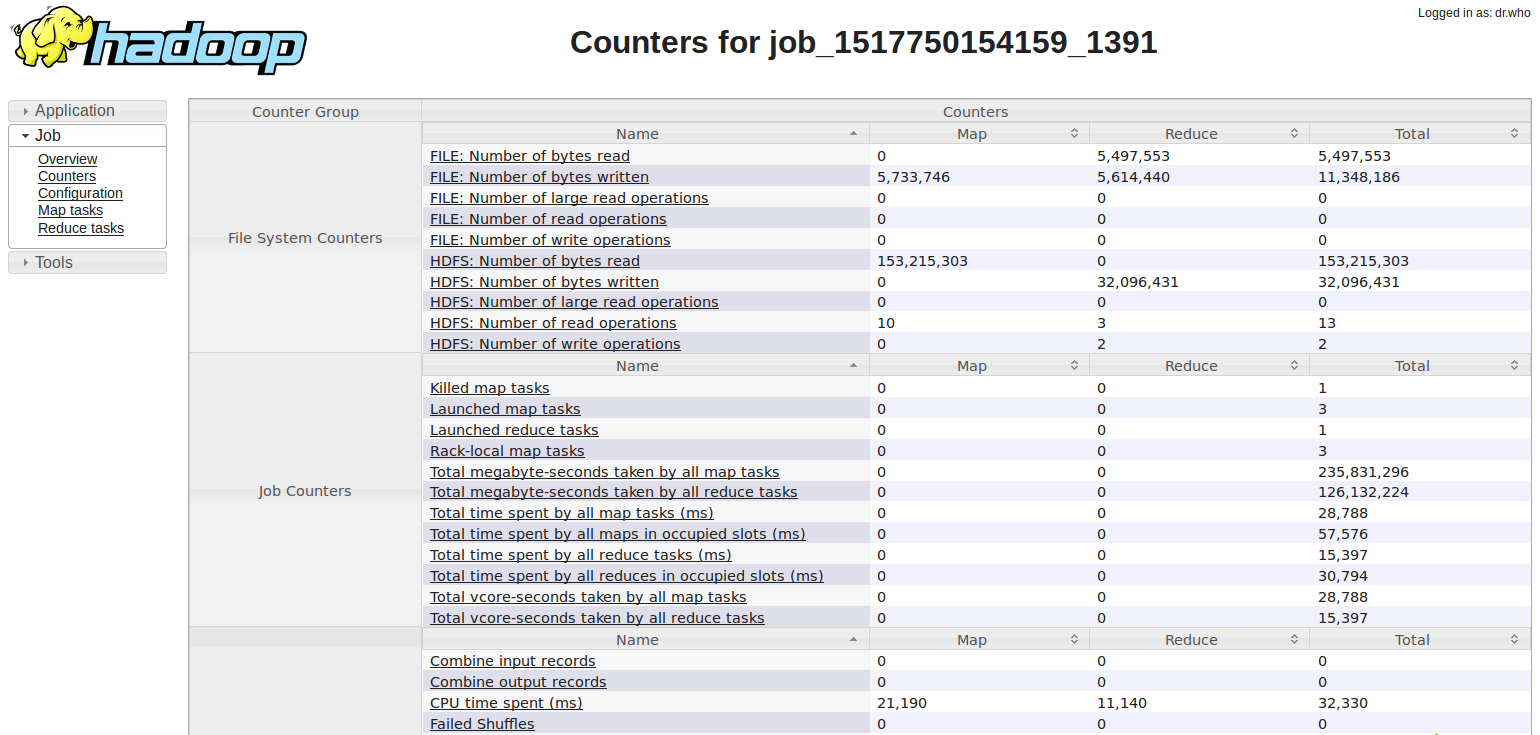
\includegraphics[width=\textwidth]{pic/391_exp_norm_counters.png}
	\caption{exp\_norm Counters}
\end{figure}

\begin{figure}[H]
	\centering
	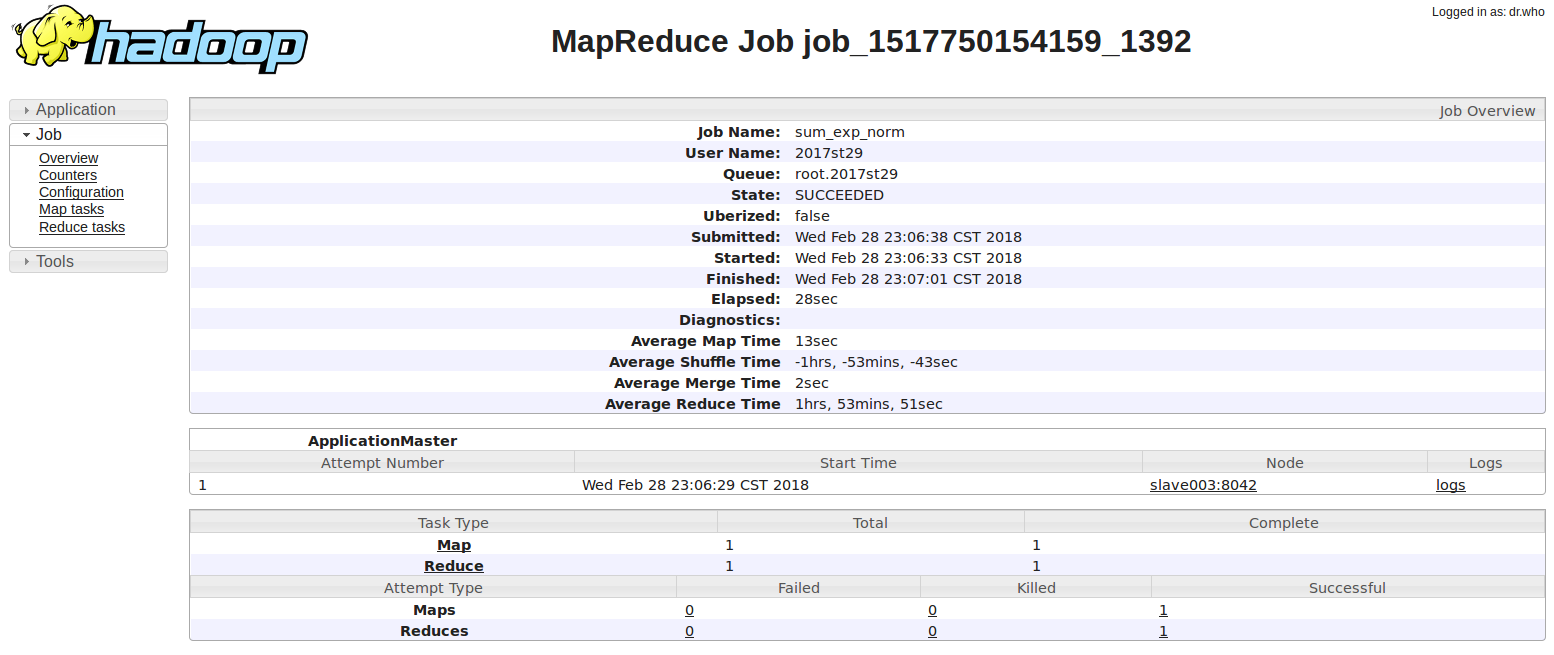
\includegraphics[width=\textwidth]{pic/392_sum_exp_norm_job.png}
	\caption{sum\_exp\_norm Job}
\end{figure}
\begin{figure}[H]
	\centering
	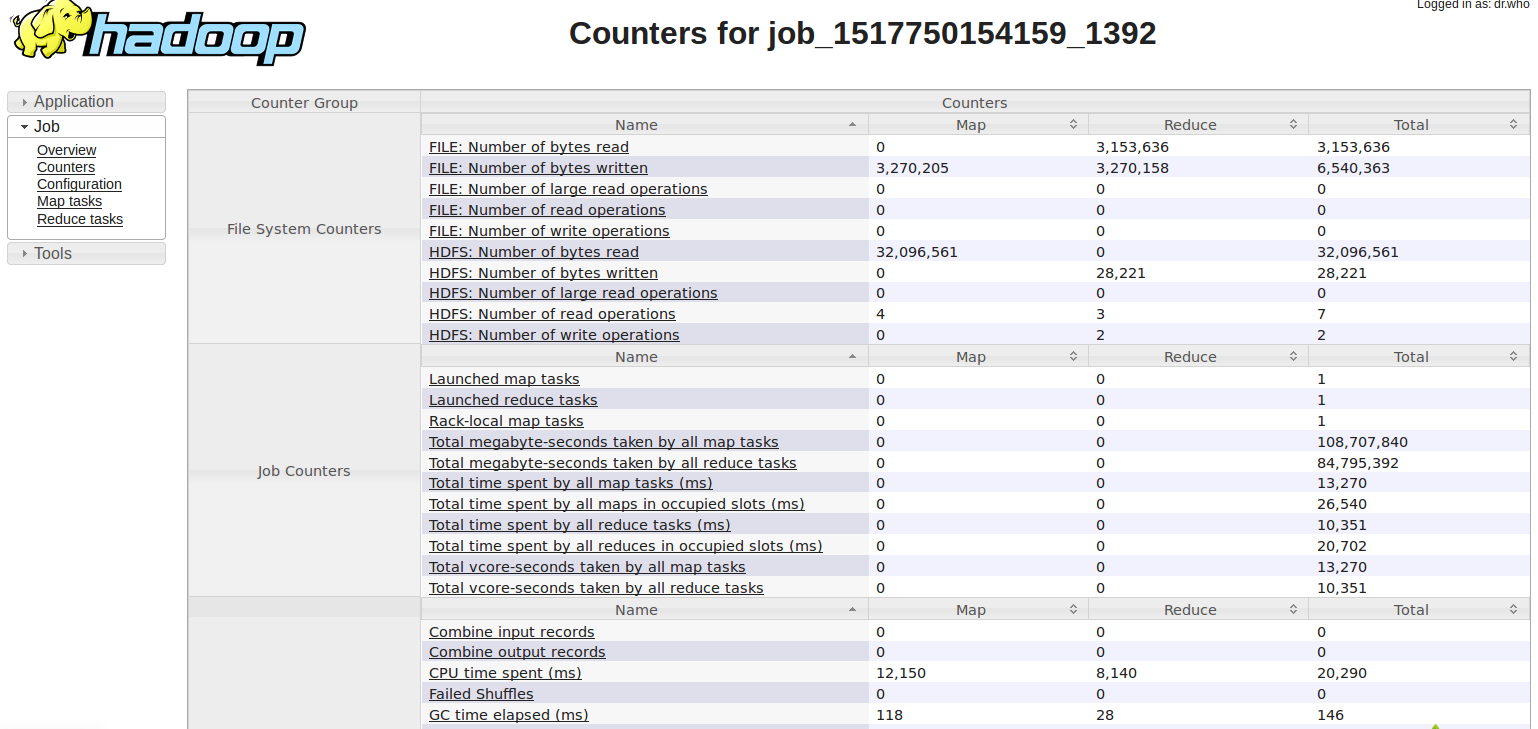
\includegraphics[width=\textwidth]{pic/392_sum_exp_norm_counters.png}
	\caption{sum\_exp\_norm Counters}
\end{figure}

\begin{figure}[H]
	\centering
	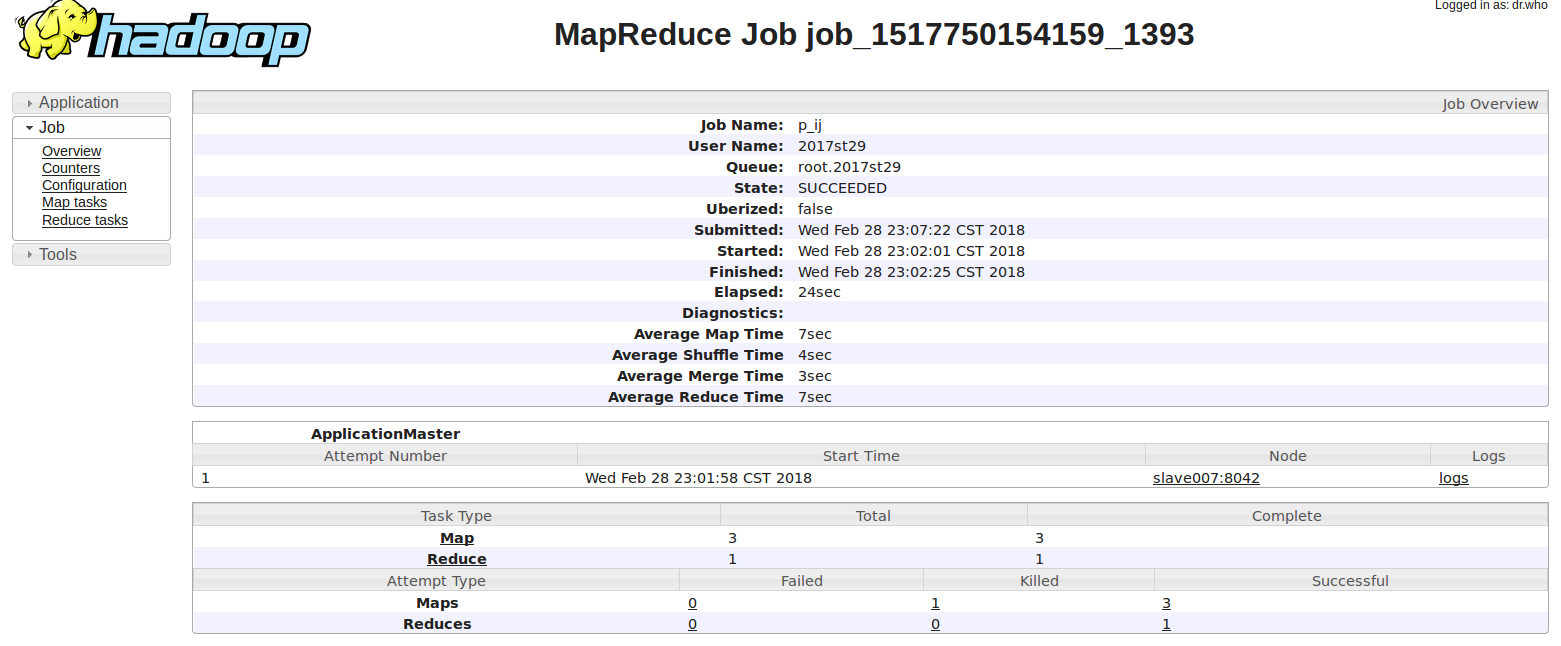
\includegraphics[width=\textwidth]{pic/393_p_ij_job.png}
	\caption{p\_ij Job}
\end{figure}
\begin{figure}[H]
	\centering
	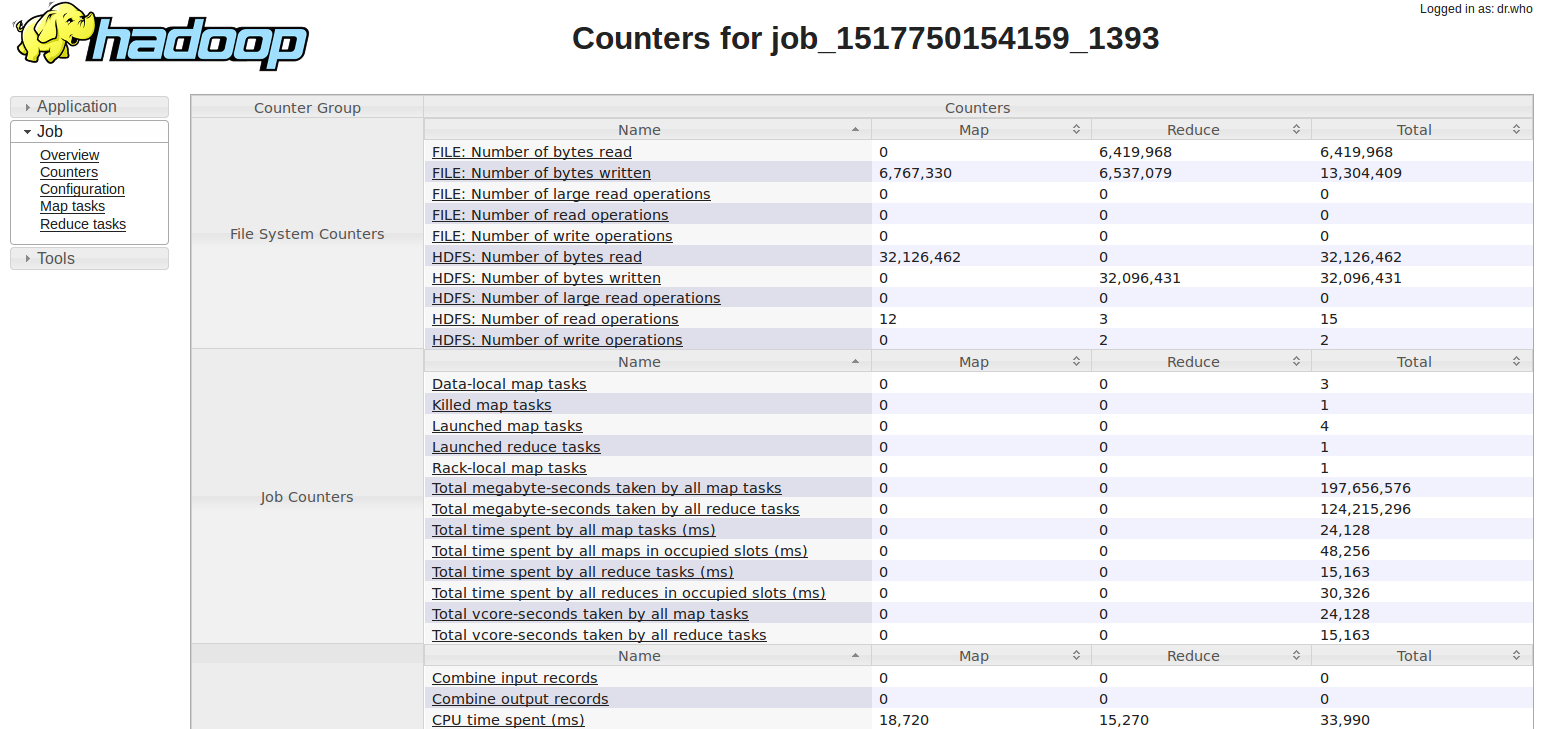
\includegraphics[width=\textwidth]{pic/393_p_ij_counters.png}
	\caption{p\_ij Counters}
\end{figure}

\begin{figure}[H]
	\centering
	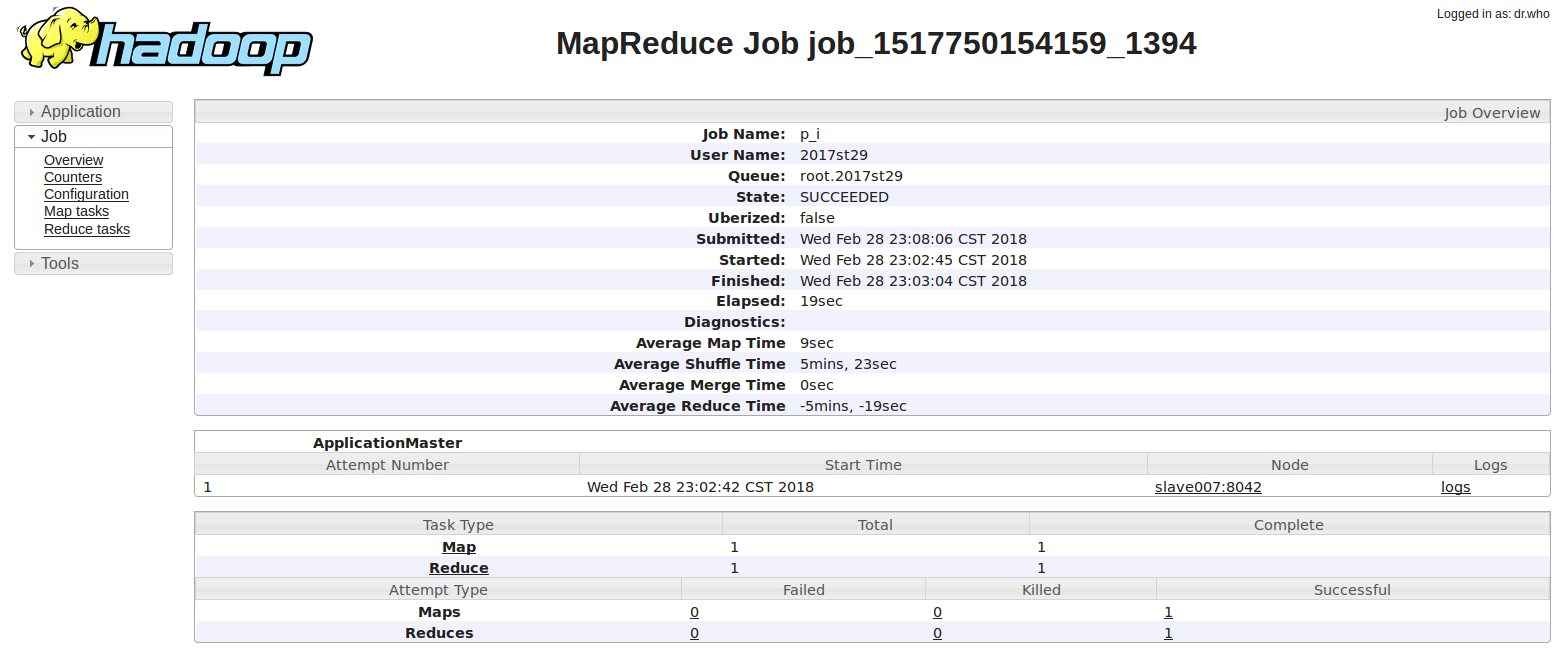
\includegraphics[width=\textwidth]{pic/394_p_i_job.png}
	\caption{p\_i Job}
\end{figure}
\begin{figure}[H]
	\centering
	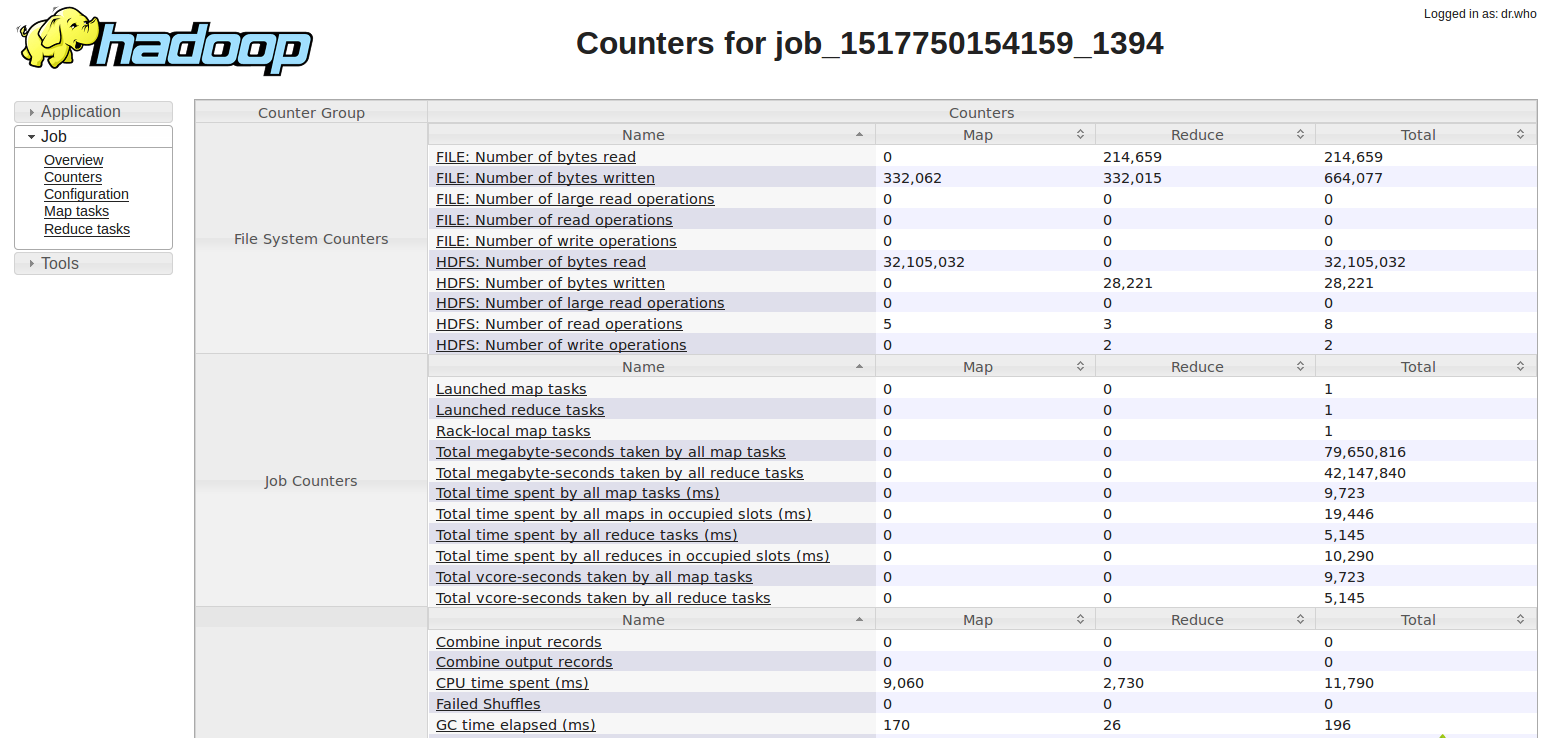
\includegraphics[width=\textwidth]{pic/394_p_i_counters.png}
	\caption{p\_i Counters}
\end{figure}

\begin{figure}[H]
	\centering
	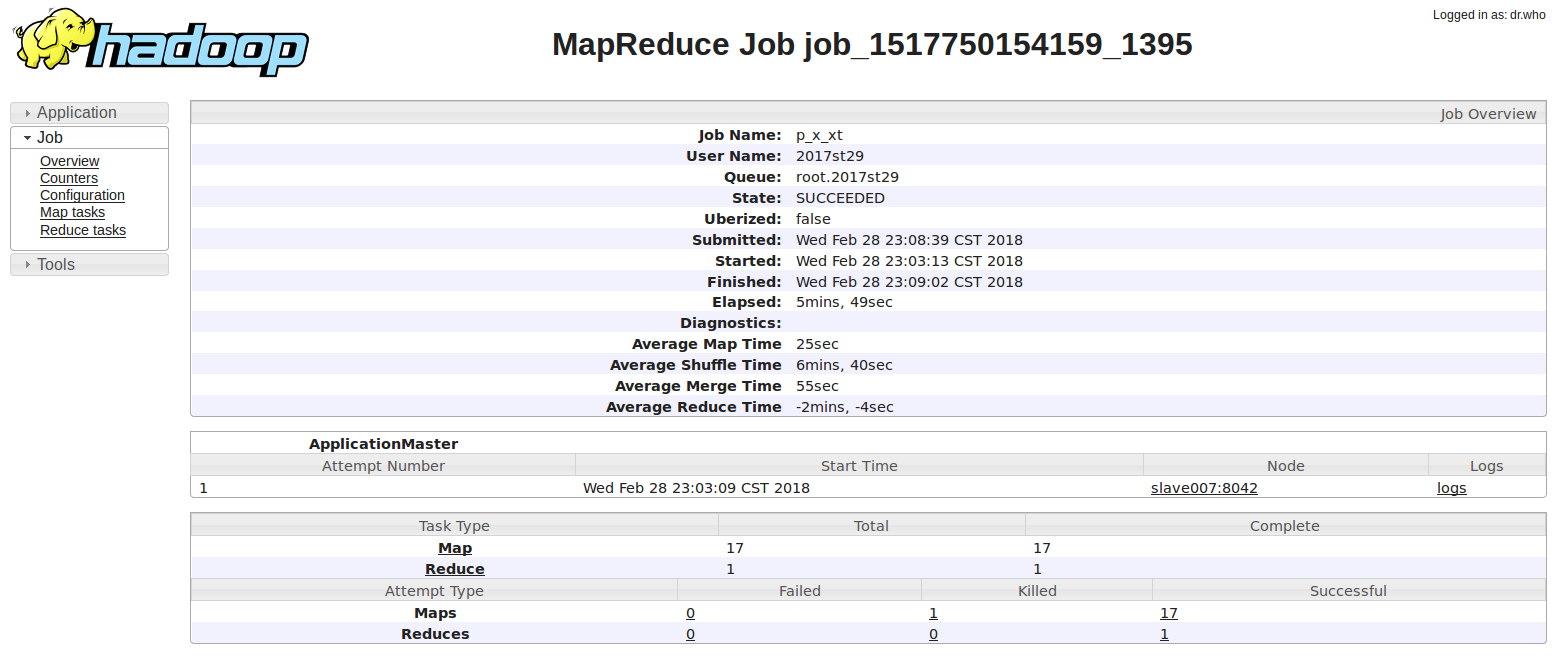
\includegraphics[width=\textwidth]{pic/395_p_x_xt_job.png}
	\caption{p\_x\_xt Job}
\end{figure}
\begin{figure}[H]
	\centering
	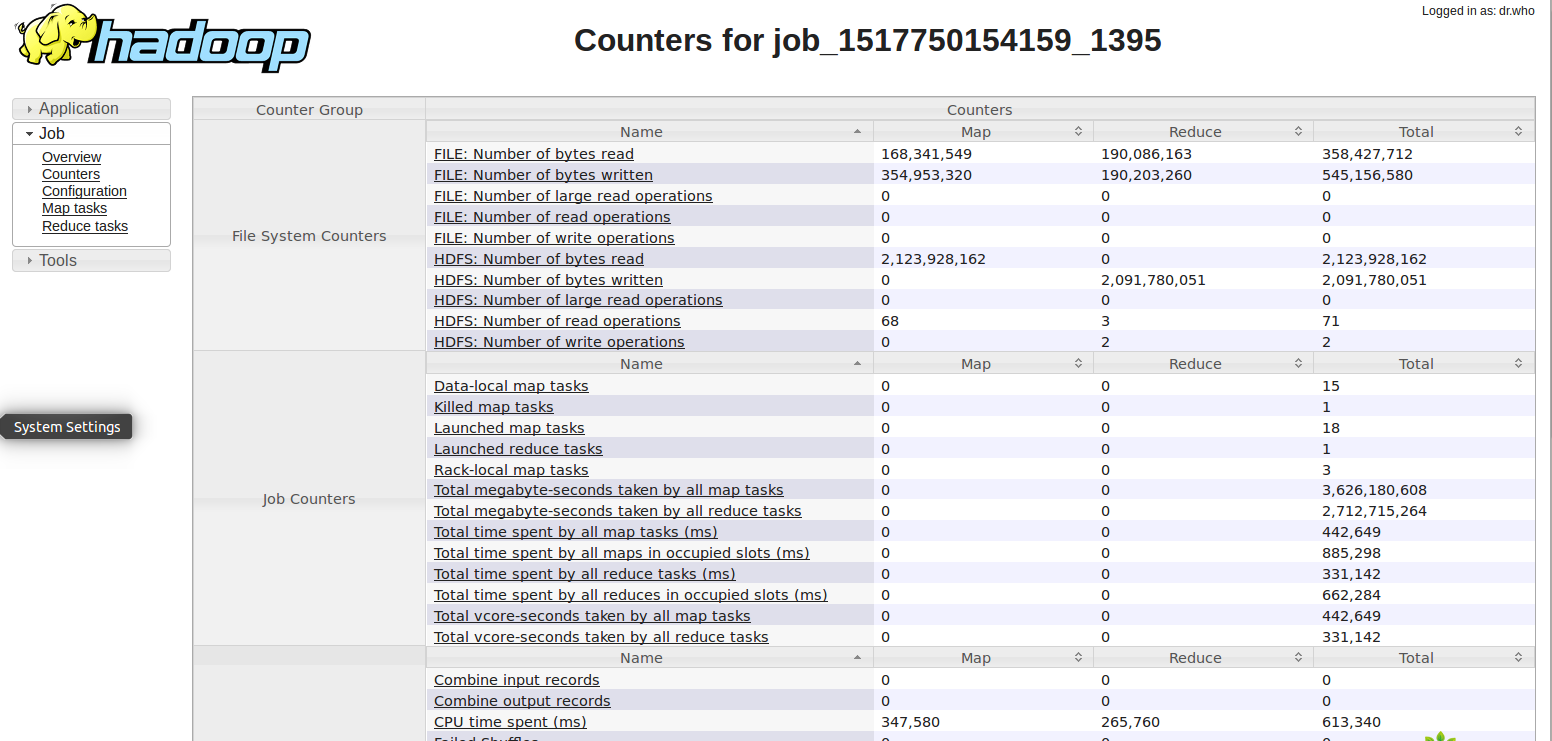
\includegraphics[width=\textwidth]{pic/395_p_x_xt_counters.png}
	\caption{p\_x\_xt Counters}
\end{figure}

\begin{figure}[H]
	\centering
	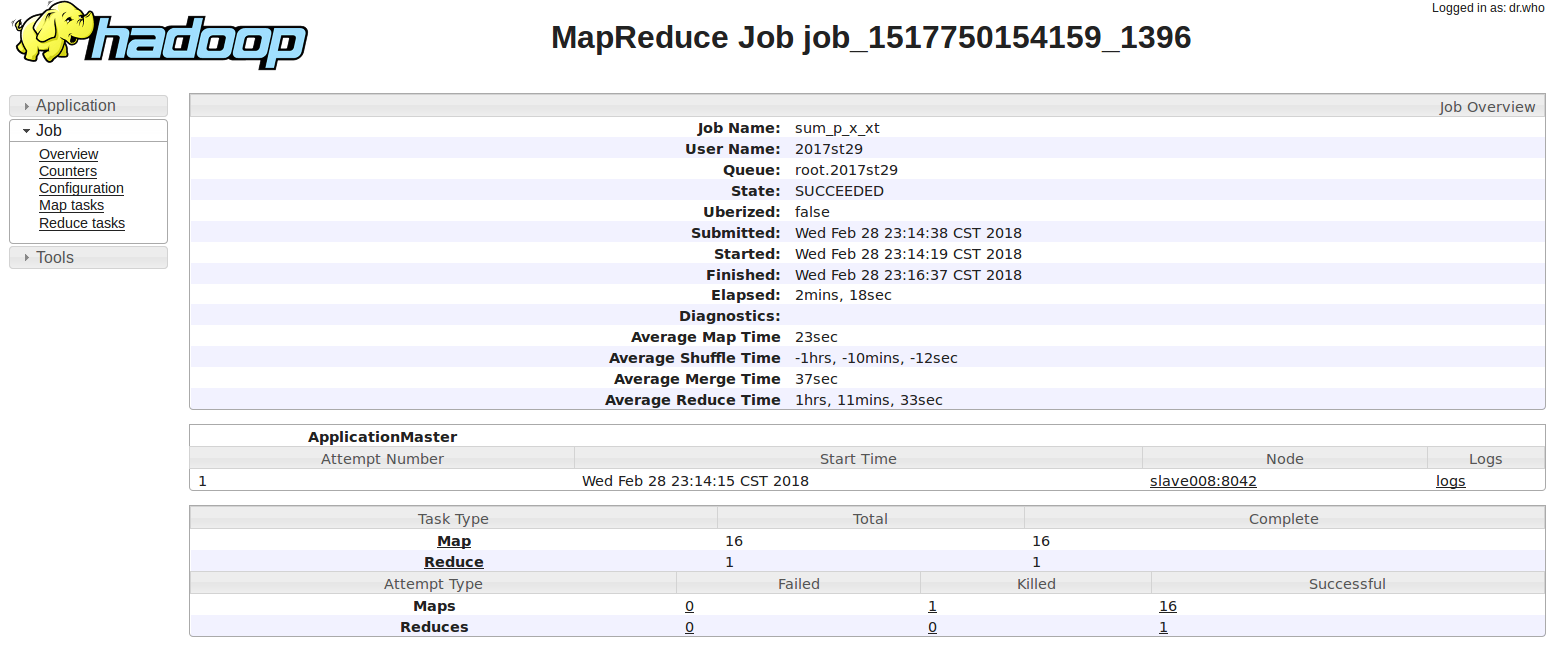
\includegraphics[width=\textwidth]{pic/396_sum_p_x_xt_job.png}
	\caption{sum\_p\_x\_xt Job}
\end{figure}
\begin{figure}[H]
	\centering
	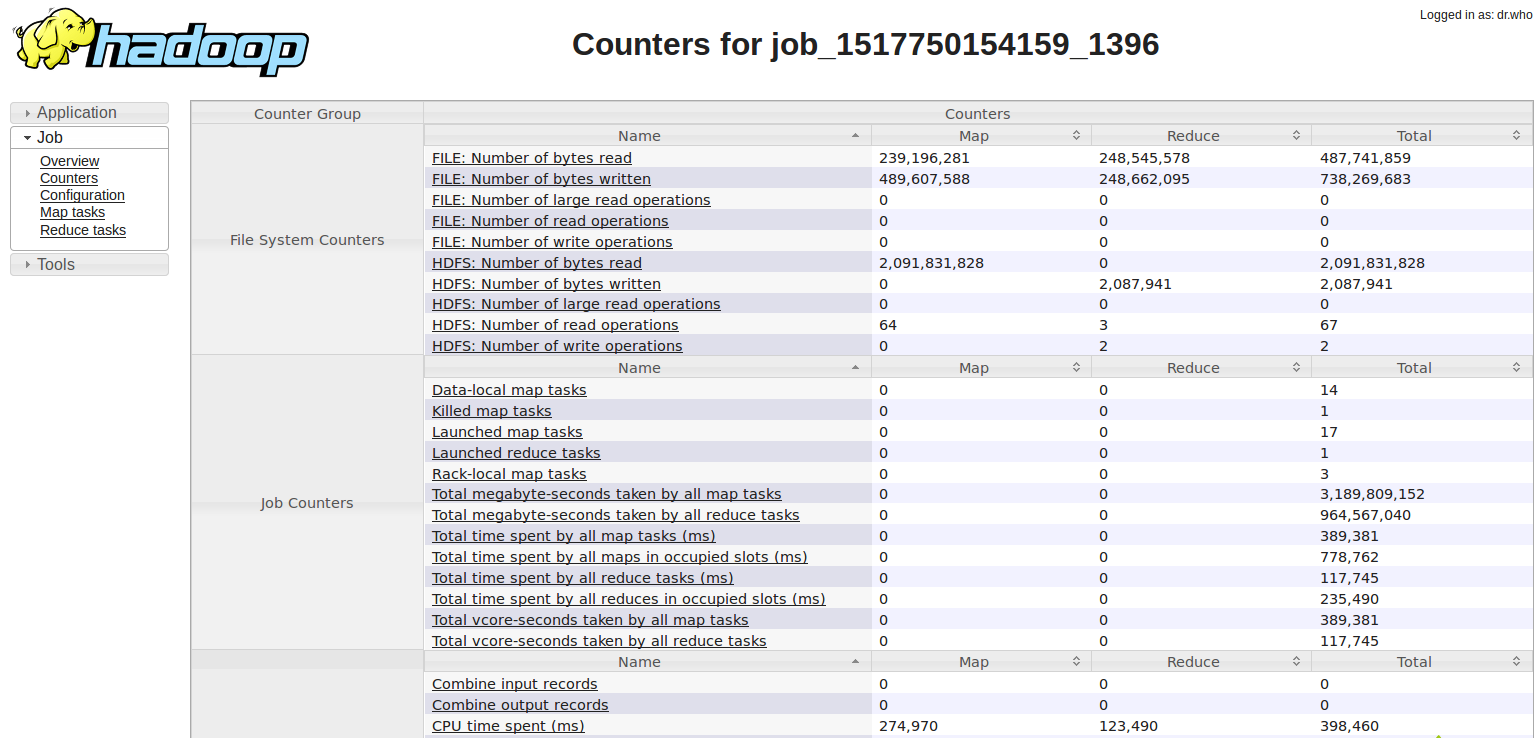
\includegraphics[width=\textwidth]{pic/396_sum_p_x_xt_counters.png}
	\caption{sum\_p\_x\_xt Counters}
\end{figure}

\begin{figure}[H]
	\centering
	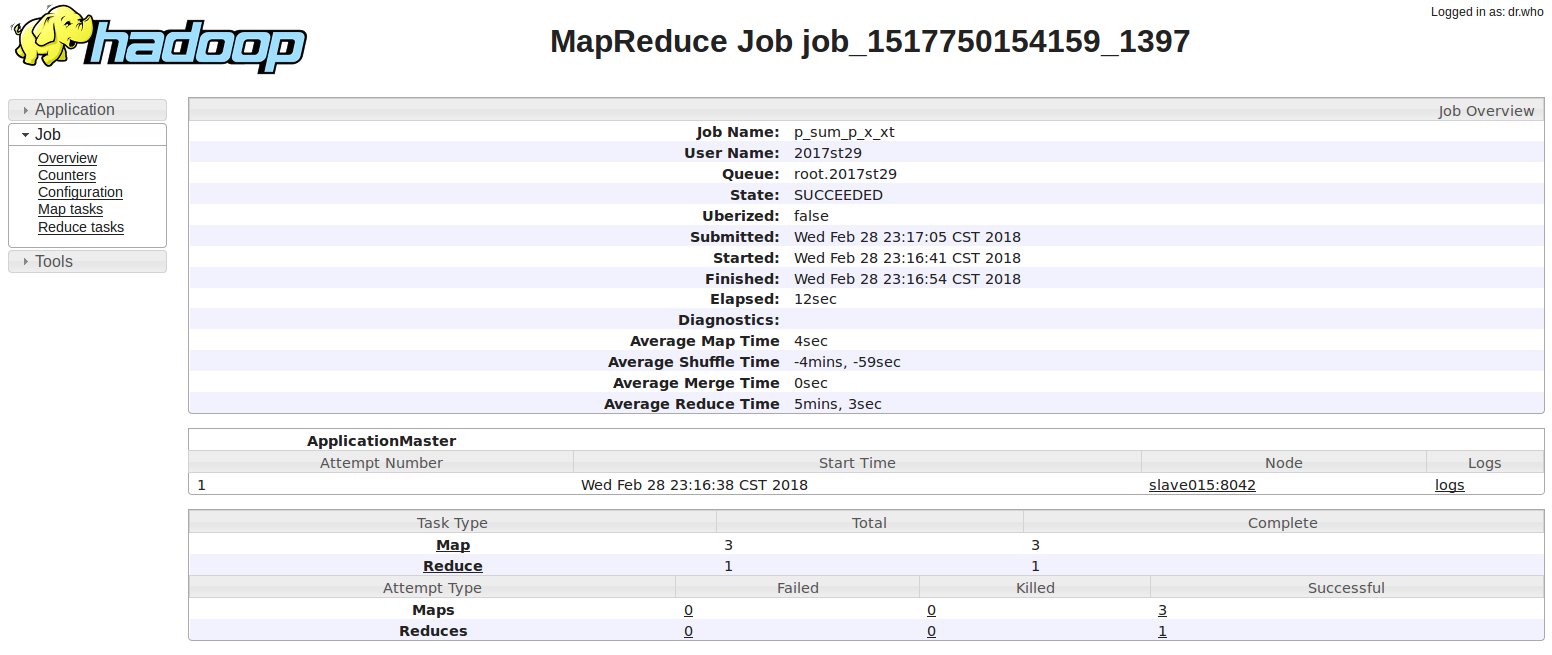
\includegraphics[width=\textwidth]{pic/397_p_sum_p_x_xt_job.png}
	\caption{p\_sum\_p\_x\_xt Job}
\end{figure}
\begin{figure}[H]
	\centering
	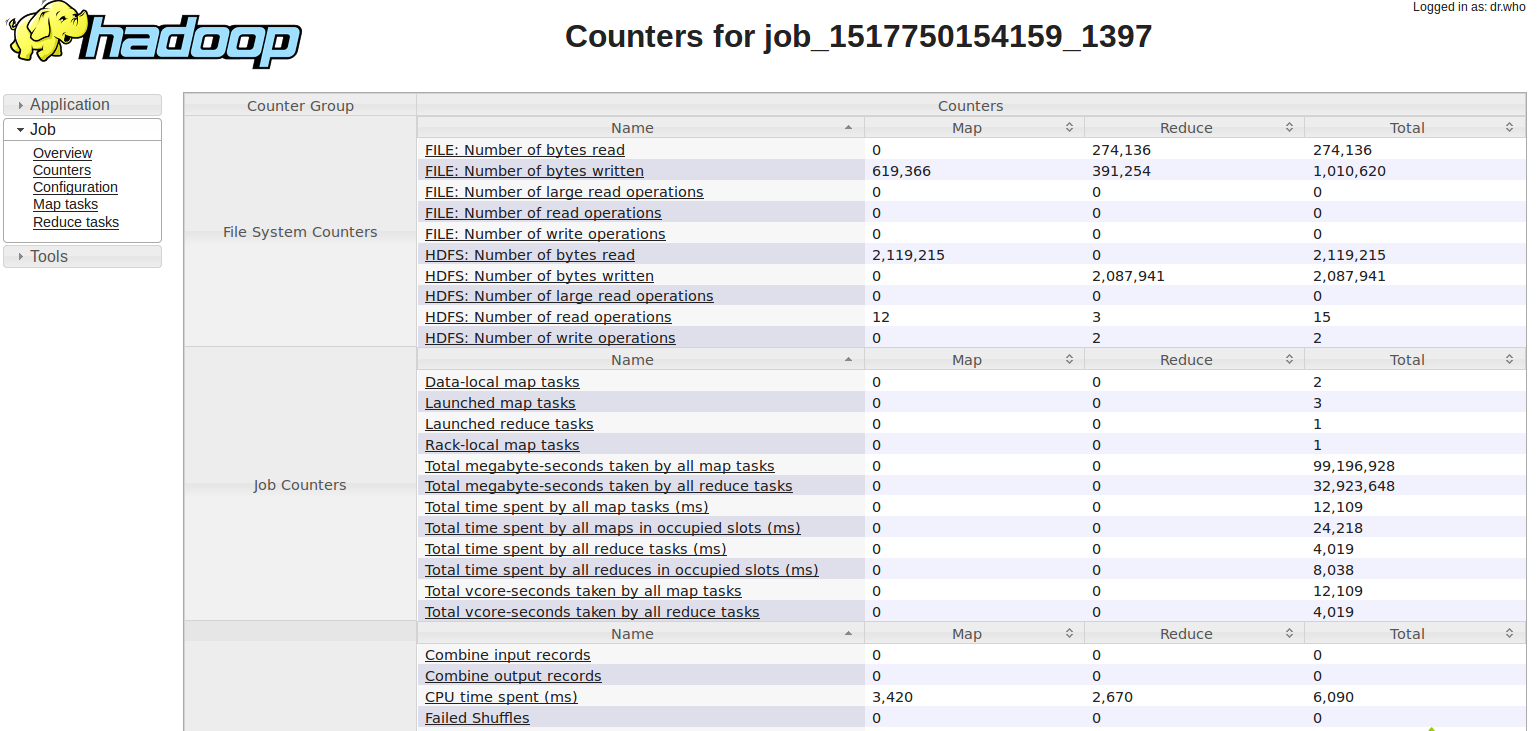
\includegraphics[width=\textwidth]{pic/397_p_sum_p_x_xt_counters.png}
	\caption{p\_sum\_p\_x\_xt Counters}
\end{figure}

\begin{figure}[H]
	\centering
	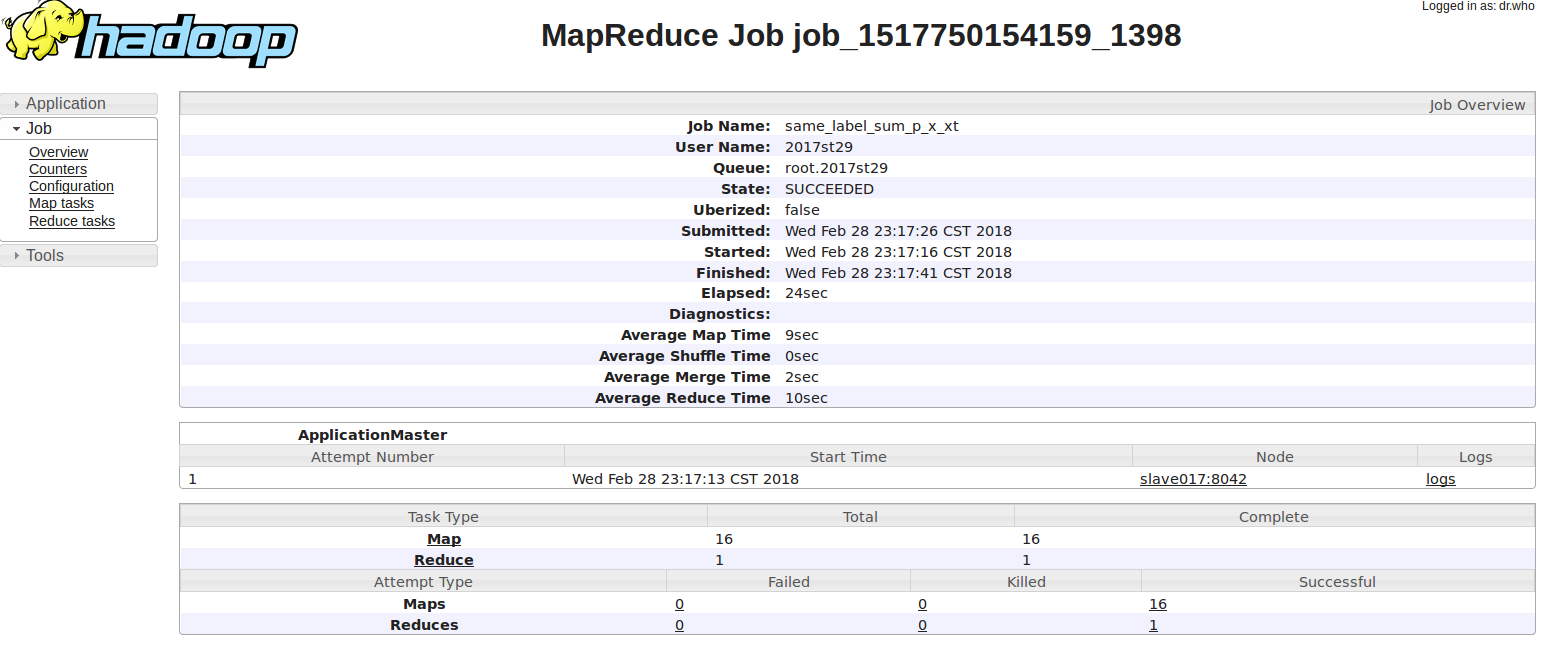
\includegraphics[width=\textwidth]{pic/398_same_label_sum_p_x_xt_job.png}
	\caption{same\_label\_sum\_p\_x\_xt Job}
\end{figure}
\begin{figure}[H]
	\centering
	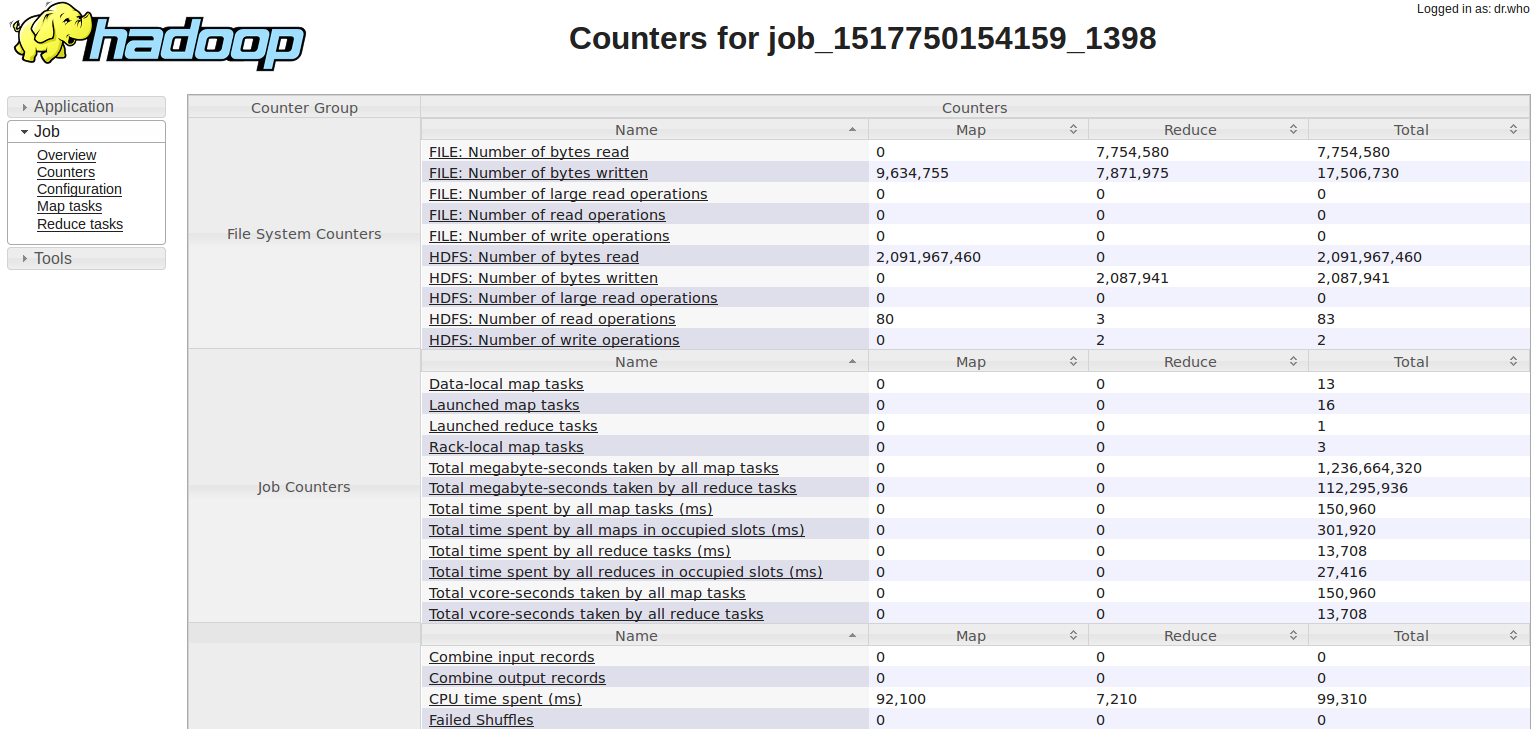
\includegraphics[width=\textwidth]{pic/398_same_label_sum_p_x_xt_counters.png}
	\caption{same\_label\_sum\_p\_x\_xt Counters}
\end{figure}

\begin{figure}[H]
	\centering
	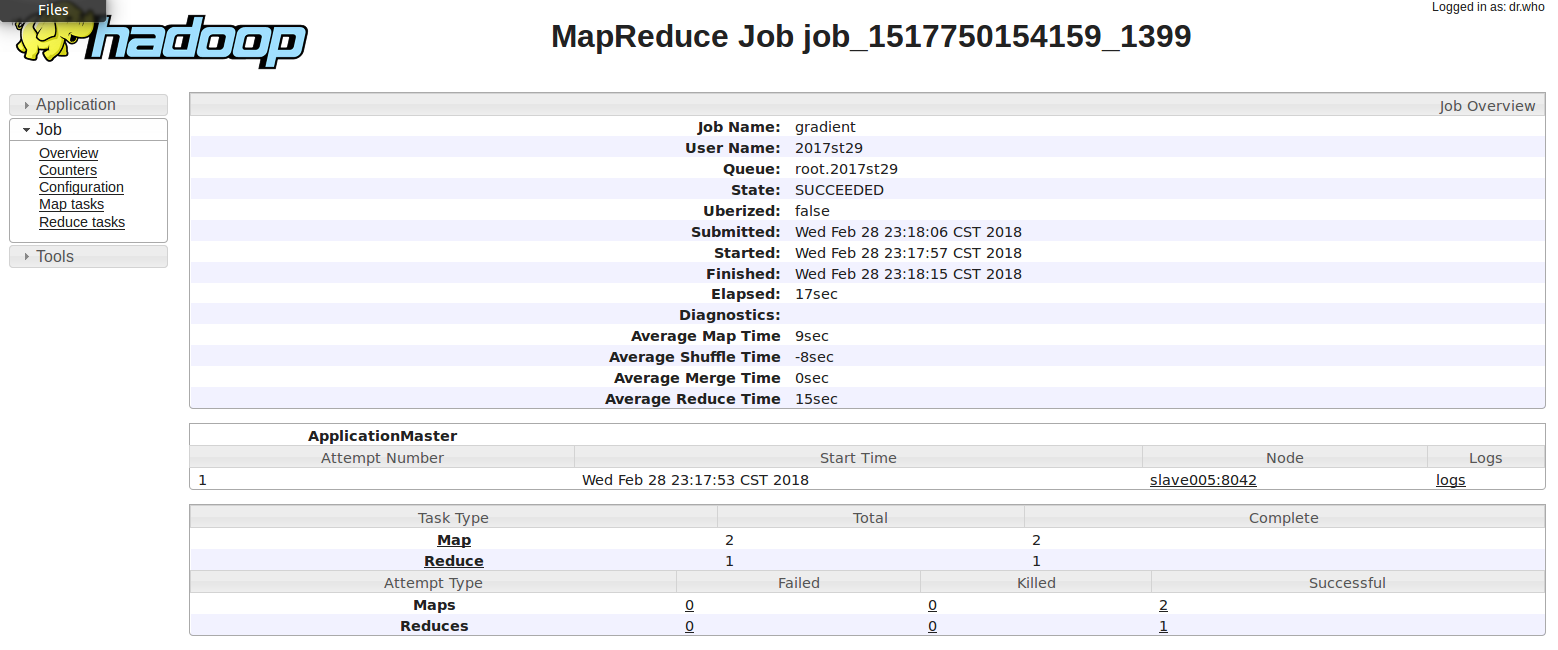
\includegraphics[width=\textwidth]{pic/399_gradient_job.png}
	\caption{gradient Job}
\end{figure}
\begin{figure}[H]
	\centering
	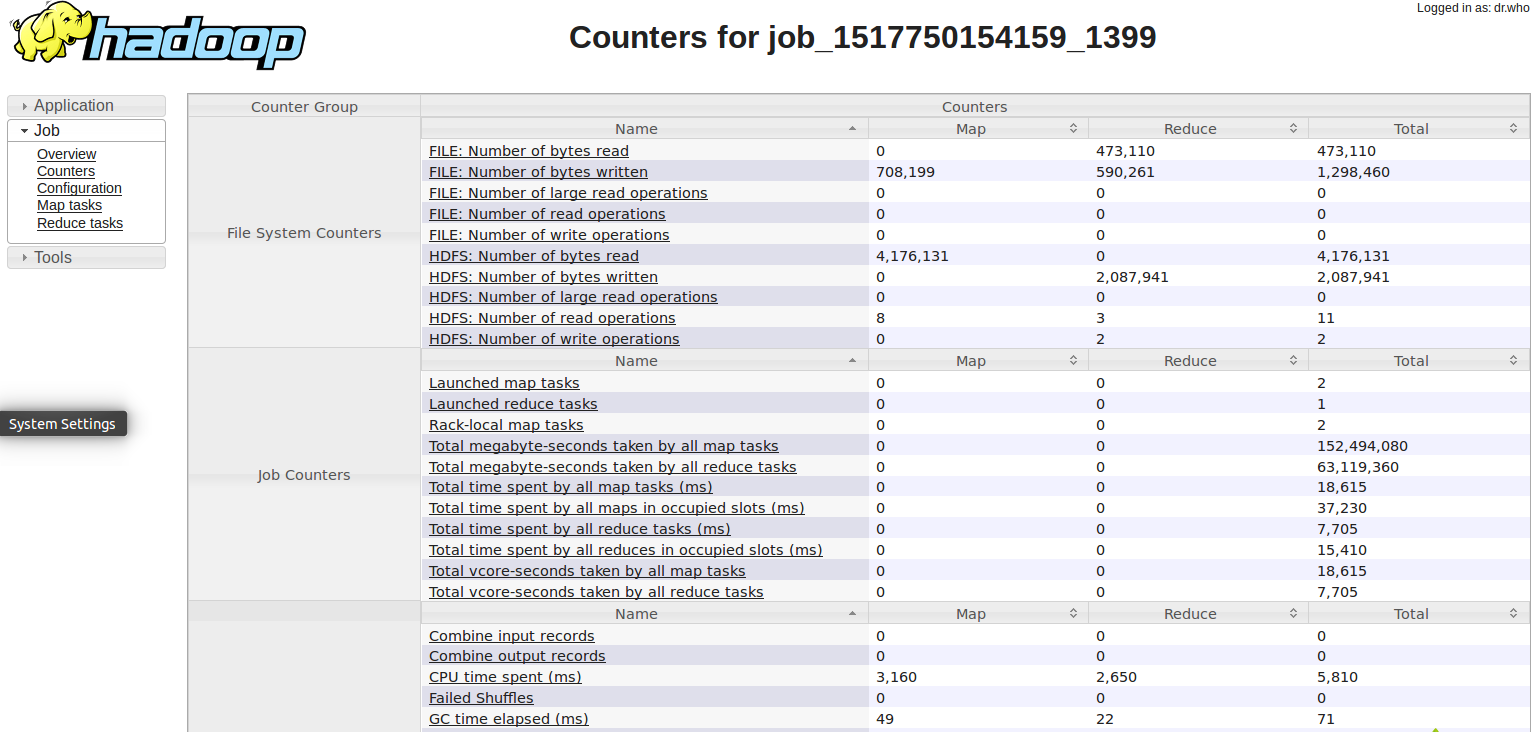
\includegraphics[width=\textwidth]{pic/399_gradient_counters.png}
	\caption{gradient Counters}
\end{figure}

\begin{figure}[H]
	\centering
	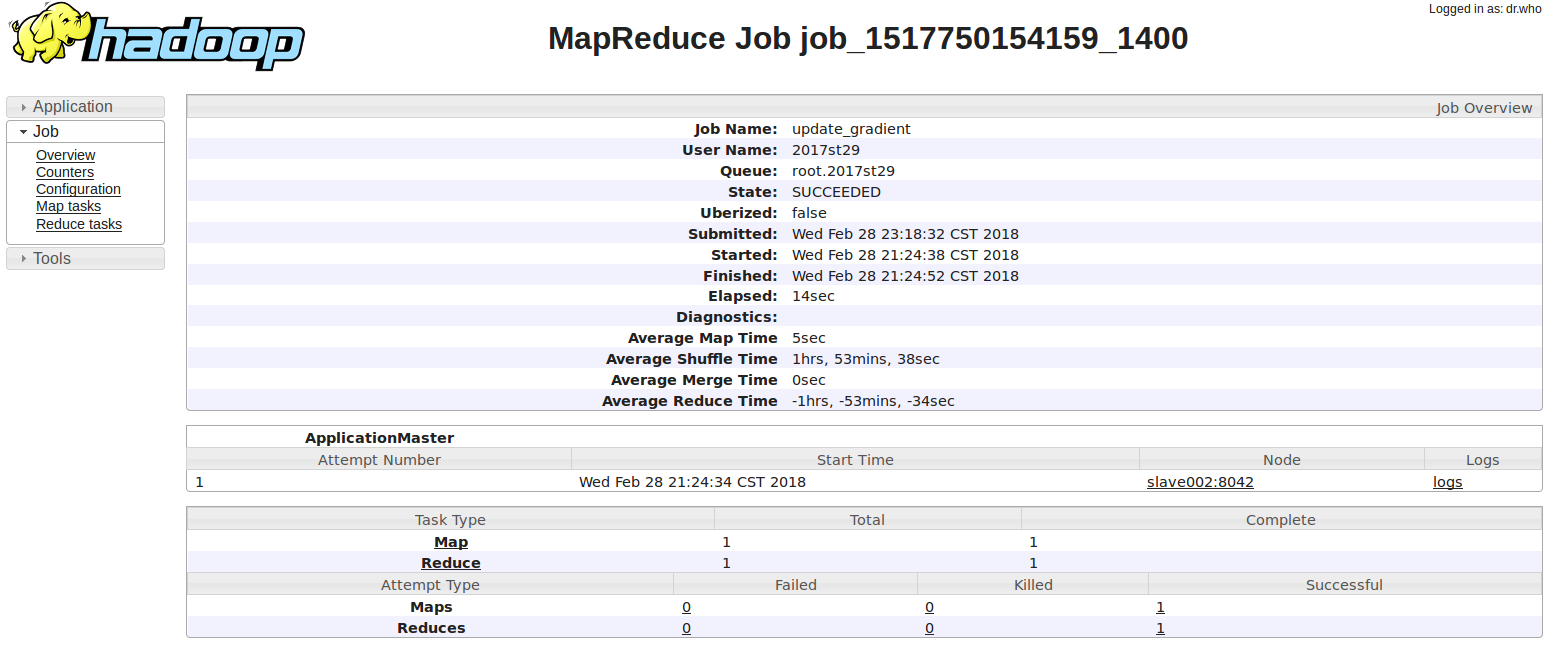
\includegraphics[width=\textwidth]{pic/400_update_gradient_job.png}
	\caption{update\_gradient Job}
\end{figure}
\begin{figure}[H]
	\centering
	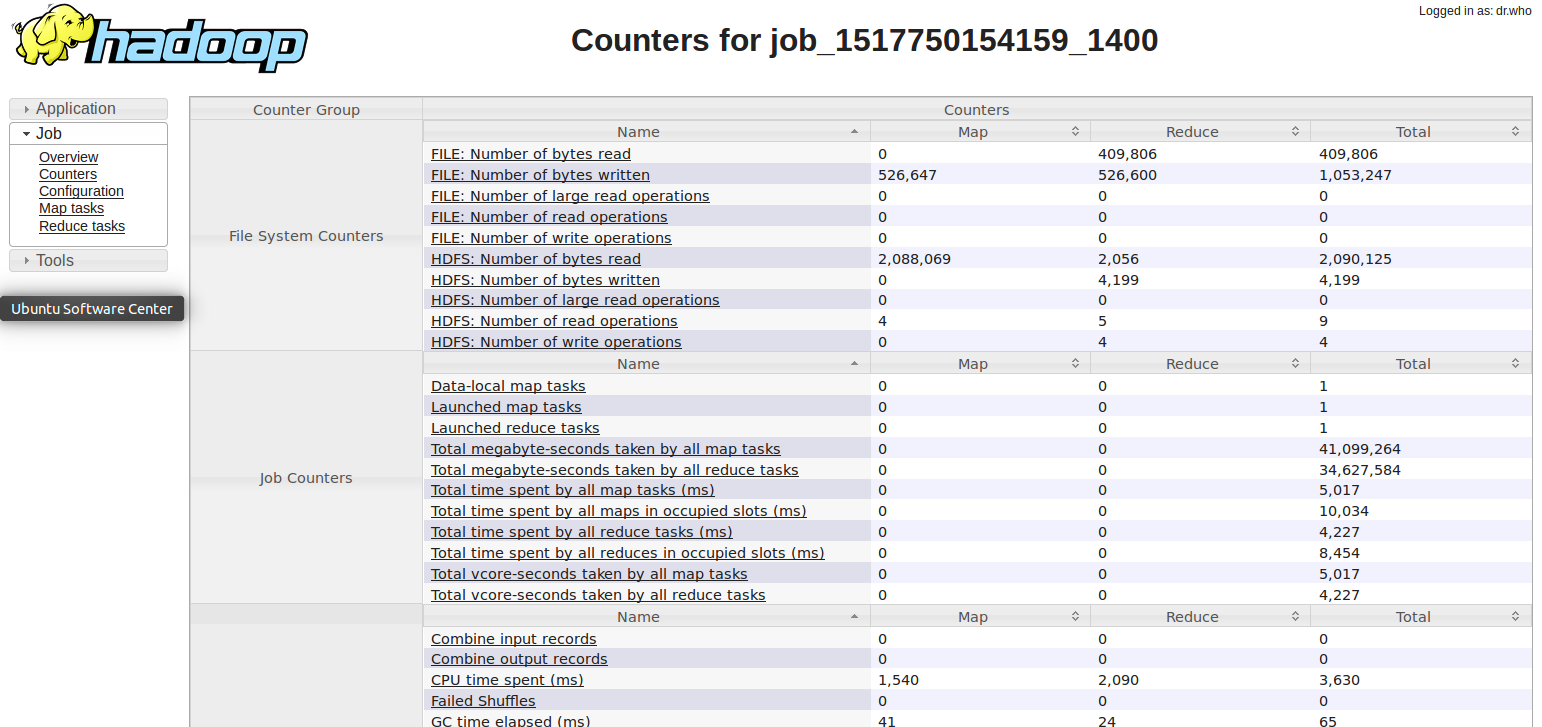
\includegraphics[width=\textwidth]{pic/400_update_gradient_counters.png}
	\caption{update\_gradient Counters}
\end{figure}

\section*{总结}

通过本次实验,我们尝试解决在机器学习课程中遇到的问题:
在数据量较大和数据维度较高的情况下,如何高效地进行梯度下降计算。
这一目标可进一步归结为如何将Tensor运算并行化。
在本次实验中,我们将Tensor进一步拆分为矩阵的列表,
并使用MapReduce设计了不同的矩阵运算算子来处理NCA中需要用到的矩阵运算。
通过将数据分布到集群上处理,我们可以执行单机难以处理的计算,
并利用并行化的优势加快其执行速度。

我们使用Apache的commons-math3作为矩阵运算库,
但是它仅仅是针对简单的矩阵运算而设计的,
并且没有对运算速度作太多的优化,
可能在单个矩阵操作的运算速度上不及numpy之类;
但是我们可以很方便地用高效的矩阵运算库来替代当前的实现,从而获得性能上的提升。

在实现NCA的过程中,我们其实构建了一个简单的并行矩阵处理的框架。
在以后如果遇到类似的计算问题,
我们可以在此基础上通过实现新的矩阵运算算子和对这些算子进行组合来解决。
这确实为我们解决问题提供了新的思路。

\nocite{*}
\bibliography{final}

\end{document}

